

\documentclass{article}
\usepackage[utf8]{inputenc}
\usepackage[utf8]{inputenc}
\usepackage[T1]{fontenc}
\usepackage[english]{babel}
\usepackage{fullpage}
\usepackage{color}
\usepackage[table]{xcolor}
\usepackage{listings}
 
\definecolor{darkWhite}{rgb}{0.94,0.94,0.94}
 
\lstset{
  aboveskip=3mm,
  belowskip=-2mm,
  backgroundcolor=\color{darkWhite},
  basicstyle=\footnotesize,
  breakatwhitespace=false,
  breaklines=true,
  captionpos=b,
  commentstyle=\color{red},
  deletekeywords={...},
  escapeinside={\%*}{*)},
  extendedchars=true,
  framexleftmargin=16pt,
  framextopmargin=3pt,
  framexbottommargin=6pt,
  frame=tb,
  keepspaces=true,
  keywordstyle=\color{blue},
  language=C,
  literate=
  {²}{{\textsuperscript{2}}}1
  {⁴}{{\textsuperscript{4}}}1
  {⁶}{{\textsuperscript{6}}}1
  {⁸}{{\textsuperscript{8}}}1
  {€}{{\euro{}}}1
  {é}{{\'e}}1
  {è}{{\`{e}}}1
  {ê}{{\^{e}}}1
  {ë}{{\¨{e}}}1
  {É}{{\'{E}}}1
  {Ê}{{\^{E}}}1
  {û}{{\^{u}}}1
  {ù}{{\`{u}}}1
  {â}{{\^{a}}}1
  {à}{{\`{a}}}1
  {á}{{\'{a}}}1
  {ã}{{\~{a}}}1
  {Á}{{\'{A}}}1
  {Â}{{\^{A}}}1
  {Ã}{{\~{A}}}1
  {ç}{{\c{c}}}1
  {Ç}{{\c{C}}}1
  {õ}{{\~{o}}}1
  {ó}{{\'{o}}}1
  {ô}{{\^{o}}}1
  {Õ}{{\~{O}}}1
  {Ó}{{\'{O}}}1
  {Ô}{{\^{O}}}1
  {î}{{\^{i}}}1
  {Î}{{\^{I}}}1
  {í}{{\'{i}}}1
  {Í}{{\~{Í}}}1,
  morekeywords={*,...},
  numbers=left,
  numbersep=10pt,
  numberstyle=\tiny\color{black},
  rulecolor=\color{black},
  showspaces=false,
  showstringspaces=false,
  showtabs=false,
  stepnumber=1,
  stringstyle=\color{gray},
  tabsize=4,
  title=\lstname,
}
\usepackage{graphicx}
\graphicspath{ {./images/} }
\title{HAI804I – Analyse et Traitement d'Images}
\author{Fabien Caballero }

\begin{document}  

\maketitle
    \tableofcontents

\newpage

\section{Expansion dynamique}

\subsection{BraZeLow.pgm}
\begin{figure}[h]
\centerline{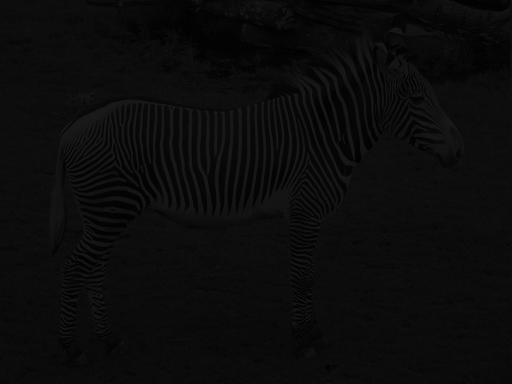
\includegraphics[scale=0.5]{./rendus/BraZeLow.png}}
\caption{BraZeLow.pgm image d'origine}
\end{figure}

\begin{figure}[h]
\centerline{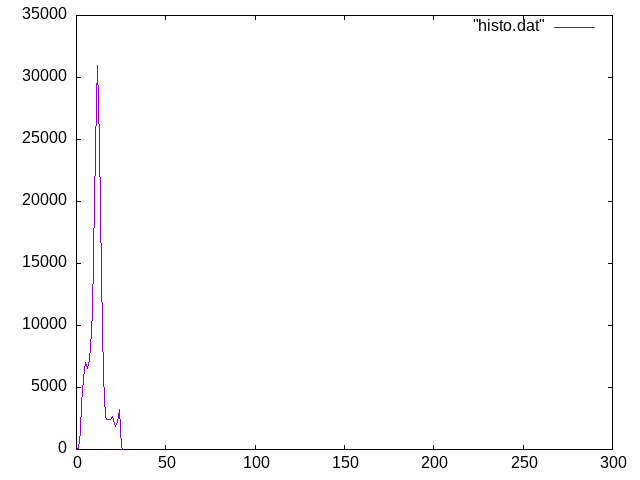
\includegraphics[scale=0.5]{./rendus/histoBraZeLowPGM.png}}
\caption{histogramme de BraZeLow.pgm}
\end{figure}

alpha= -10
beta=10

\begin{figure}[h]
\centerline{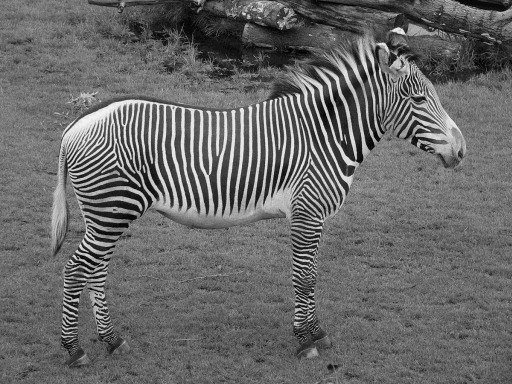
\includegraphics[scale=0.5]{./rendus/AnimalInconnu.png}}
\caption{BraZeLow'.pgm}
\end{figure}

\begin{figure}[h]
\centerline{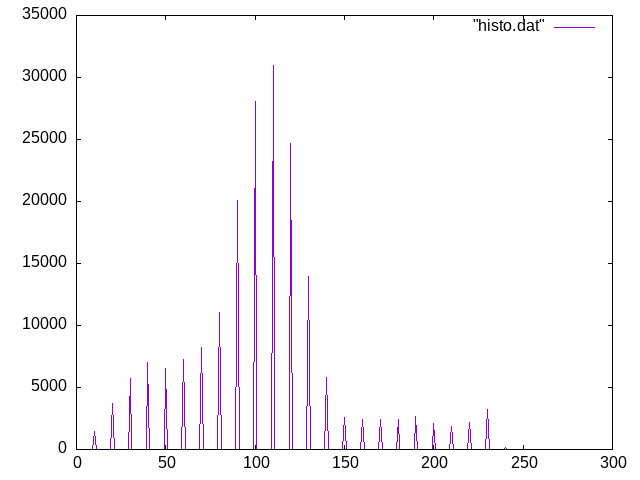
\includegraphics[scale=0.5]{./rendus/histoAnimalInconnu.png}}
\caption{histogramme BraZeLow'.pgm }
\end{figure}

\newpage
\subsection{black.ppm}
\begin{figure}[h]
\centerline{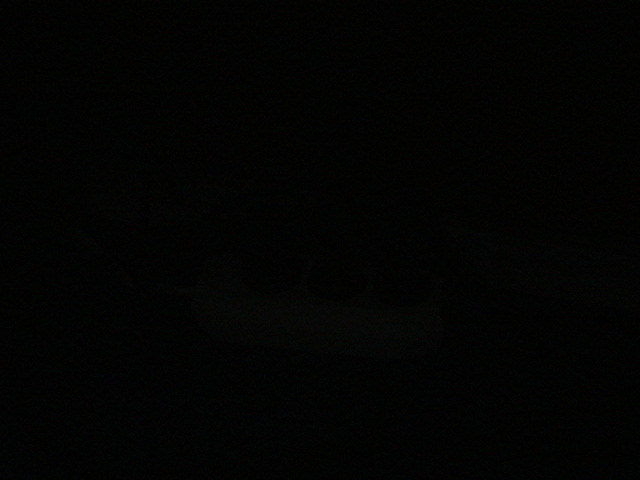
\includegraphics[scale=0.5]{./rendus/black.png}}
\caption{black.pgm }
\end{figure}

\begin{figure}[h]
\centerline{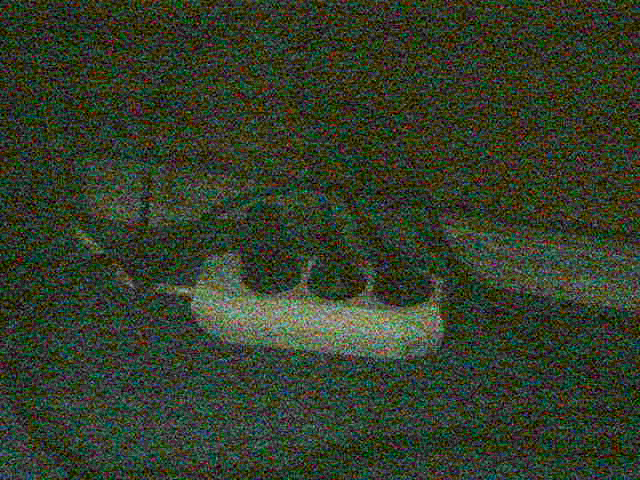
\includegraphics[scale=0.5]{./rendus/blackOut.png}}
\caption{black'.pgm }
\end{figure}

\begin{figure}[h]
% \centerline{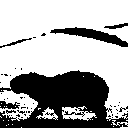
\includegraphics[scale=1.4]{./rendus/capybatapSeuil.png}}
\caption{capybara.pgm avec un seuil automatique avec la moyenne}
\end{figure}

Pour le seuillage, on parcours chaque pixel et on teste sa valeur, si celle-ci est inférieure au seuil on met à 0 (noir) ce pixel dans le tableau de l'image de sortie, sinon à 255 (blanc).

\end{document}